\chapter{Análisis Funcional}

\section{Actores}
En el software desarrollado, cada rol dentro del staff de RVA ha sido considerado como un actor diferente. Para el contexto del presente proyecto, el cargo de cada actor corresponde a su nombre, lo que quiere decir que si un actor lleva por nombre ''Administrador'', se entenderá que su cargo es ''Administrador de la comunidad de RVA''. Sólo los jugadores no cuentan con un cargo dentro de RVA.

La especificación de todos los actores se puede encontrar a continuación en la tabla TABLENUM.

\begin{center}
	\begin{tabular}{| p{3cm} | p{4.5cm} | p{4.5cm} | p{2cm} |}
		\hline
		\multicolumn{4}{|c|}{\textbf{Actores}} \\
		\hline
		\multicolumn{1}{|c|}{\textbf{Actor}} & \multicolumn{1}{|c|}{\textbf{Función}} & \multicolumn{1}{|c|}{\textbf{Conocimientos}} & \multicolumn{1}{|c|}{\textbf{Privilegio}}\\
		\hline
		{\textbf{Administrador}} & Cumple con todas las funciones dentro de la comunidad como mantener autos, pistas, sesiones y manejo general del software. Configura el software para el resto de los usuarios. & Requiere conocimiento sobre como funciona el sistema en su totalidad, comprendiendo también el contexto en el que funciona RVA como comunidad. & Máximo. \\ \hline
		{\textbf{Organizador}} & Cumple con funciones específicamente relacionadas al manejo de sesiones multijugador y el procesamiento de los puntajes. & Requiere conocimiento específico de como subir archivos de sesión a la aplicación web, y un contexto general de como funciona RVA. & Intermedio (módulo de sesiones).\\ \hline
		{\textbf{Moderador}} & Utiliza las funciones específicas de manejo de usuarios, tal como la edición de perfiles o aplicación de infracciones. & Requiere conocimientos que se limitan al manejo de usuarios dentro de la web. & Intermedio (manejo de usuarios).\\ \hline
		{\textbf{Jugador}} & Utiliza la página sólo para visualizar la información que esta ofrece. & No requiere conocimientos técnicos más allá de iniciar sesión. & Ninguno.\\ \hline
	\end{tabular}
\end{center}

\section{Diagrama de Casos de Uso}
...

\section{Modelo de Datos}
Diagrama con Modelo de datos no relacional:

\begin{center}
	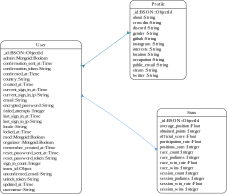
\includegraphics{datamodel1.png}
\end{center}

\begin{center}
	\includegraphics{datamodel2.png}
\end{center}


\begin{center}
	\includegraphics{datamodel3.png}
\end{center}

\begin{center}
	\includegraphics{datamodel4.png}
\end{center}

\section{Esquema de la Base de Datos}
A continuación, se describen los datos de la base de datos mediante archivos de definición de modelos de Ruby con mongoid:

\section{Diseño de Interfaz}

\section{Diseño de Arquitectura}
El proyecto, en su estado actual, hace uso de un servidor propio, el cual contiene los servicios web, bases de datos y caché. Todo en una sola máquina. Independientemente de donde se termine alojanda, la aplicación web estará disponible en ''https://rva.lat/''.

Además de esto, la planificación contempla dos servicios externos, que actualmente son proveídos por GitHub pages, los cuales sirven como repositorios de almacenamiento de datos masivos. Dichos repositorios se encargan actualmente de servir información y assets como las imágenes de las pistas y autos que la web ofrece a los usuarios:

\begin{itemize}
	\item https://tracks.rva.lat/: Repositorio de pistas de RVA.
	\item https://cars.rva.lat/: Repositorio de autos de RVA.
\end{itemize}

A continuación, se muestra un diagrama que ilustra todo el proceso de interacción entre servicios y usuarios:








Tal como se muestra en la ilustración, la arquitectura que da soporte a la aplicación web de RVA se concentra en un servidor, con dos almacenes de datos. Podemos ver que los usuarios en la práctica juegan la sesión, el host de la sesión sube el Session Log a la web, y los usuarios pueden visitar la misma web para revisar los resultados

\section{Estructura del código}
El proyecto, al ser una aplicación hecha en el framework de Ruby on Rails, sigue patrón de MVC (Model View Controller), o modelo, vista, controlador. El árbol de directorio se ve de la siguiente manera:

% IMAGEN

Todas las bases de datos dentro de MongoDB están prefijadas utilizando el término “rv”. Por ejemplo, la base de datos que almacena las colecciones de autos se llama “rv\_cars”, la de los usuarios “rv\_users”, etc.

\subsection{Backend}

%TABLA

\subsection{Frontend}

%TABLA

\section{Estado del Proyecto}
Actualmente, el proyecto se encuentra finalizado.

EXPLICAR TODO LO QUE SE TERMINÓ

Además de lo anterior, se ha programado e implementado completamente la lógica operativa interna de Re-Volt America dentro del sistema, por lo que este puede recibir archivos Session Log, procesarlos y almacenarlos correctamente, mostrando al usuario una vista interpretada de los resultados de la sesión.

PROYECCIONES?



